% Titre de la partie
\section{Mise en place de GitHub Classroom}


%%%%%%%%%%%%%%%%%%%%%%%%%%%%%%%%%%%%%%%%%%%%%%%%
%%%%%%%%%%%%%%%%%%%%%%%%%%%%%%%%%%%%%%%%%%%%%%%%
\begin{frame}
	\frametitle{Ensemble du processus}
	%\framesubtitle{}

	Il est décrit dans cette petite vidéo

	\begin{center}
		\url{https://www.youtube.com/watch?v=ChA_zph7aao}
	\end{center}


\end{frame}



%%%%%%%%%%%%%%%%%%%%%%%%%%%%%%%%%%%%%%%%%%%%%%%%
%%%%%%%%%%%%%%%%%%%%%%%%%%%%%%%%%%%%%%%%%%%%%%%%
\begin{frame}
	\frametitle{Création de l'organisation}
	%\framesubtitle{}

	\begin{center}
		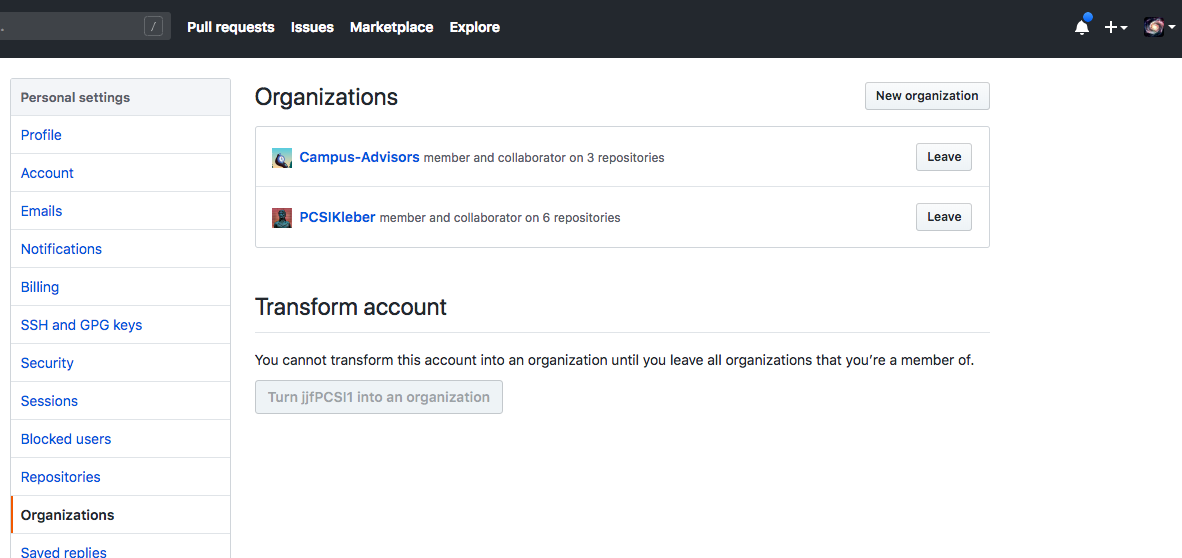
\includegraphics[width=0.8\linewidth]{figures/classroom_organization.png}
	\end{center}

	\begin{itemize}[<+->]
		\item	Depuis \url{github.com}, aller dans «Settings» (en haut à droite sur l'avatar de votre compte)

		\item Puis «Organizations» (onglet en bas à gauche)

		\item Puis «New organisation» (bouton)

	\end{itemize}

\end{frame}


%%%%%%%%%%%%%%%%%%%%%%%%%%%%%%%%%%%%%%%%%%%%%%%%
%%%%%%%%%%%%%%%%%%%%%%%%%%%%%%%%%%%%%%%%%%%%%%%%
\begin{frame}
	\frametitle{Création de la \ofg{classroom}}
	\framesubtitle{Première étape}

	Depuis \url{https://classroom.github.com/classrooms} (après s'être connecté, bien entendu), cliquer sur le bouton «New classroom» (en haut à droite)

	\begin{center}
		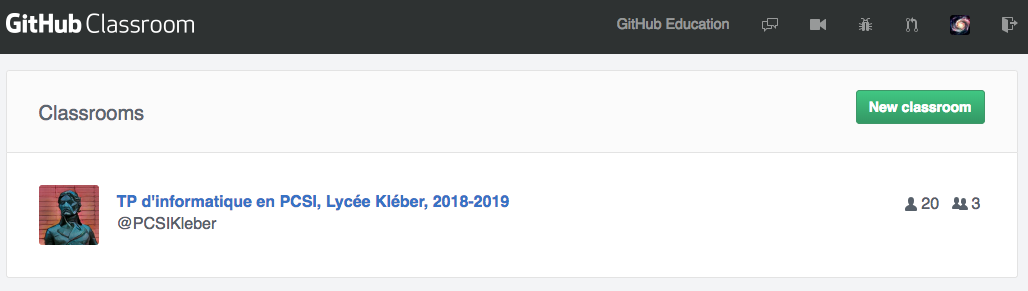
\includegraphics[width=\linewidth]{figures/classroom_new_classroom.png}
	\end{center}

\end{frame}

%%%%%%%%%%%%%%%%%%%%%%%%%%%%%%%%%%%%%%%%%%%%%%%%
%%%%%%%%%%%%%%%%%%%%%%%%%%%%%%%%%%%%%%%%%%%%%%%%
\begin{frame}
	\frametitle{Création de la \ofg{classroom}}
	\framesubtitle{Sélection de l'organization}

	Sélectionner l'«organization» adéquate

	\begin{center}
		
\includegraphics[width=\linewidth]{figures/classroom_select_organization.png}
	\end{center}

\end{frame}

%%%%%%%%%%%%%%%%%%%%%%%%%%%%%%%%%%%%%%%%%%%%%%%%
%%%%%%%%%%%%%%%%%%%%%%%%%%%%%%%%%%%%%%%%%%%%%%%%
\begin{frame}
	\frametitle{Création de la \ofg{classroom}}
	\framesubtitle{Nomination}

	Donner un nom explicite à la classroom

	\begin{center}
		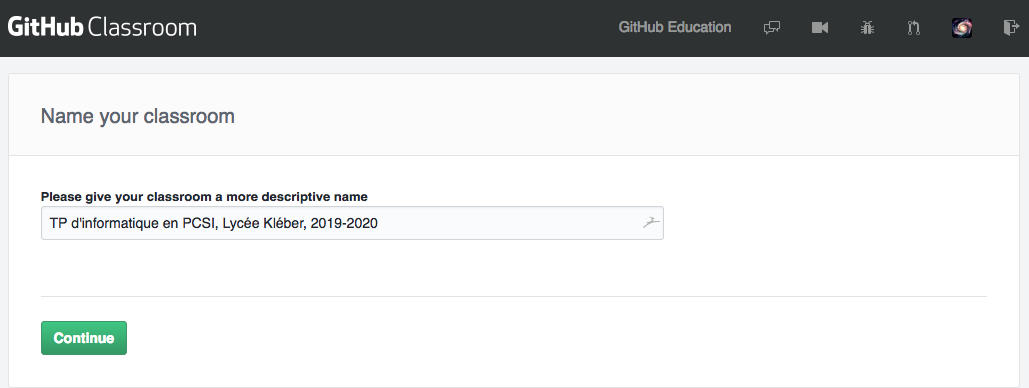
\includegraphics[width=\linewidth]{figures/classroom_naming.png}
	\end{center}

\end{frame}

%%%%%%%%%%%%%%%%%%%%%%%%%%%%%%%%%%%%%%%%%%%%%%%%
% Deuxième diapo
%%%%%%%%%%%%%%%%%%%%%%%%%%%%%%%%%%%%%%%%%%%%%%%%
\begin{frame}
	\frametitle{Création de la \ofg{classroom}}
	\framesubtitle{Invitation d'autres administrateurs}

	%Inscrivez vos collègues à votre organization et donnez-leur le lien vers la classroom

	\begin{center}
		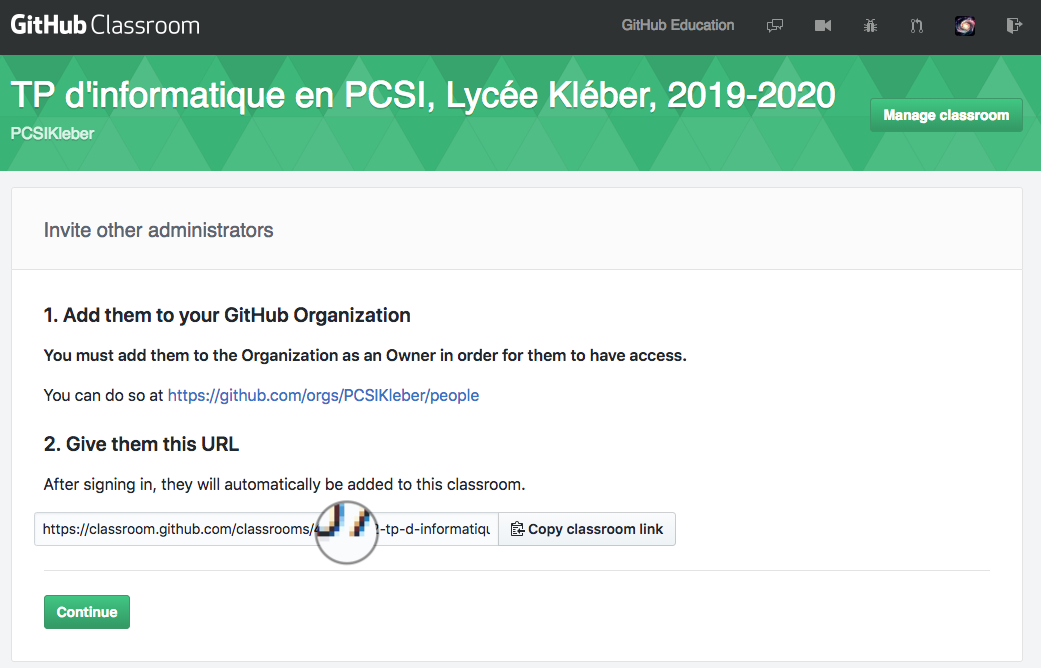
\includegraphics[width=\linewidth]{figures/classroom_invite_admin.png}
	\end{center}

\end{frame}

%%%%%%%%%%%%%%%%%%%%%%%%%%%%%%%%%%%%%%%%%%%%%%%%
% Deuxième diapo
%%%%%%%%%%%%%%%%%%%%%%%%%%%%%%%%%%%%%%%%%%%%%%%%
\begin{frame}
	\frametitle{Création de la \ofg{classroom}}
	\framesubtitle{Préparation du roster}

	%Inscrivez vos collègues à votre organization et donnez-leur le lien vers la classroom

	\begin{center}
		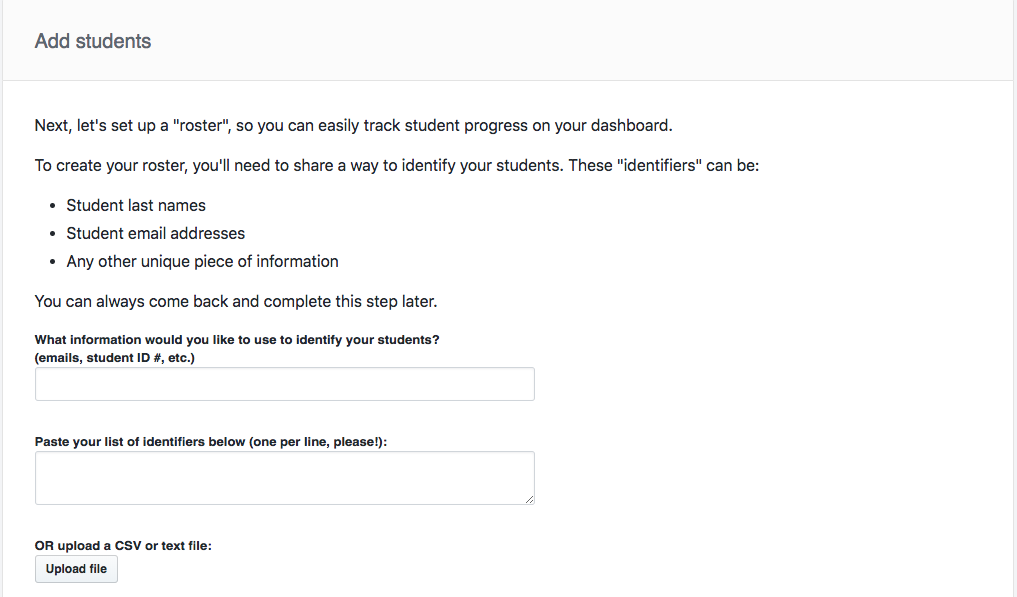
\includegraphics[width=\linewidth]{figures/classroom_roster.png}
	\end{center}

\end{frame}

%%%%%%%%%%%%%%%%%%%%%%%%%%%%%%%%%%%%%%%%%%%%%%%%
%%%%%%%%%%%%%%%%%%%%%%%%%%%%%%%%%%%%%%%%%%%%%%%%
\begin{frame}
	\frametitle{Premier «Assignment»}
	\framesubtitle{Création}

	%Inscrivez vos collègues à votre organization et donnez-leur le lien vers la classroom

	\begin{center}
		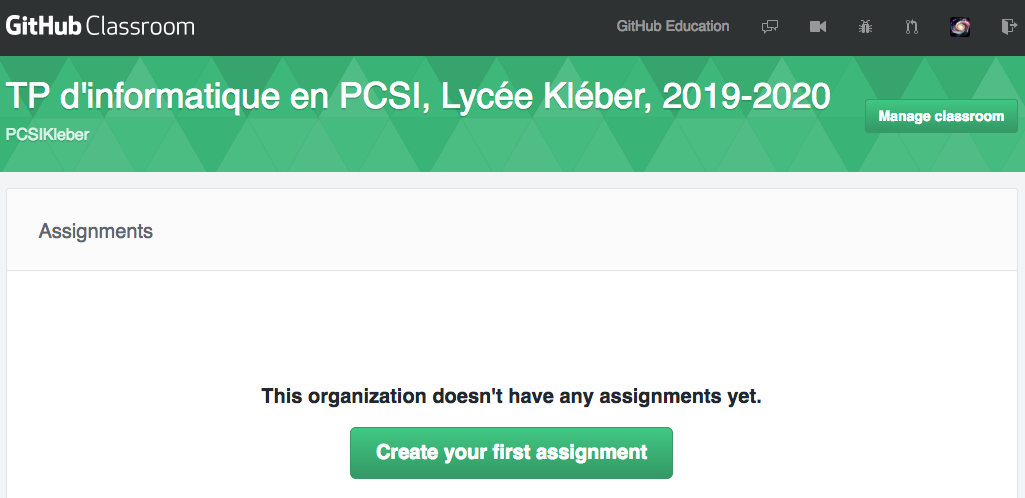
\includegraphics[width=\linewidth]{figures/classroom_assignment_creation.png}
	\end{center}

\end{frame}

%%%%%%%%%%%%%%%%%%%%%%%%%%%%%%%%%%%%%%%%%%%%%%%%
%%%%%%%%%%%%%%%%%%%%%%%%%%%%%%%%%%%%%%%%%%%%%%%%
\begin{frame}
	\frametitle{Premier «Assignment»}
	\framesubtitle{Type}

	%Inscrivez vos collègues à votre organization et donnez-leur le lien vers la classroom

	\begin{center}
		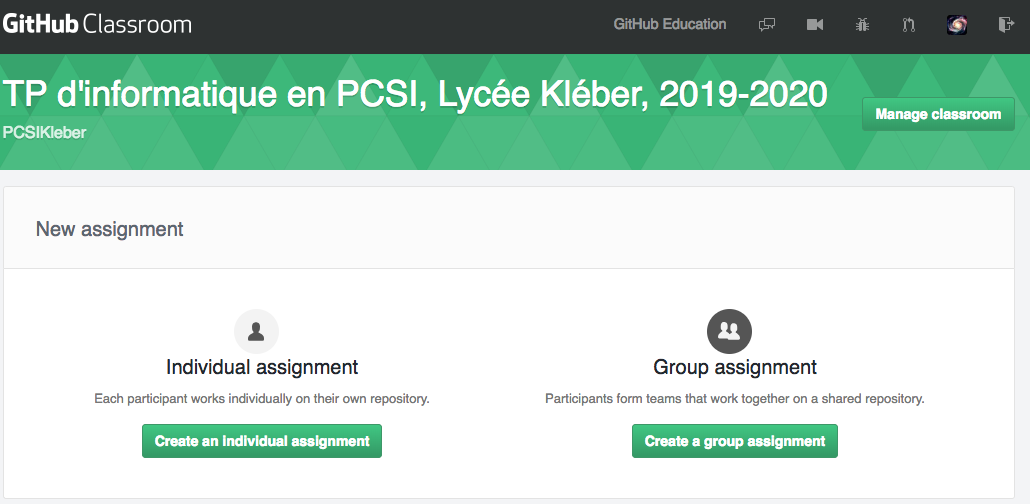
\includegraphics[width=\linewidth]{figures/classroom_assignment_type.png}
	\end{center}

\end{frame}

%%%%%%%%%%%%%%%%%%%%%%%%%%%%%%%%%%%%%%%%%%%%%%%%
%%%%%%%%%%%%%%%%%%%%%%%%%%%%%%%%%%%%%%%%%%%%%%%%
\begin{frame}
	\frametitle{Premier «Assignment»}
	\framesubtitle{Réglages}

	\begin{center}
		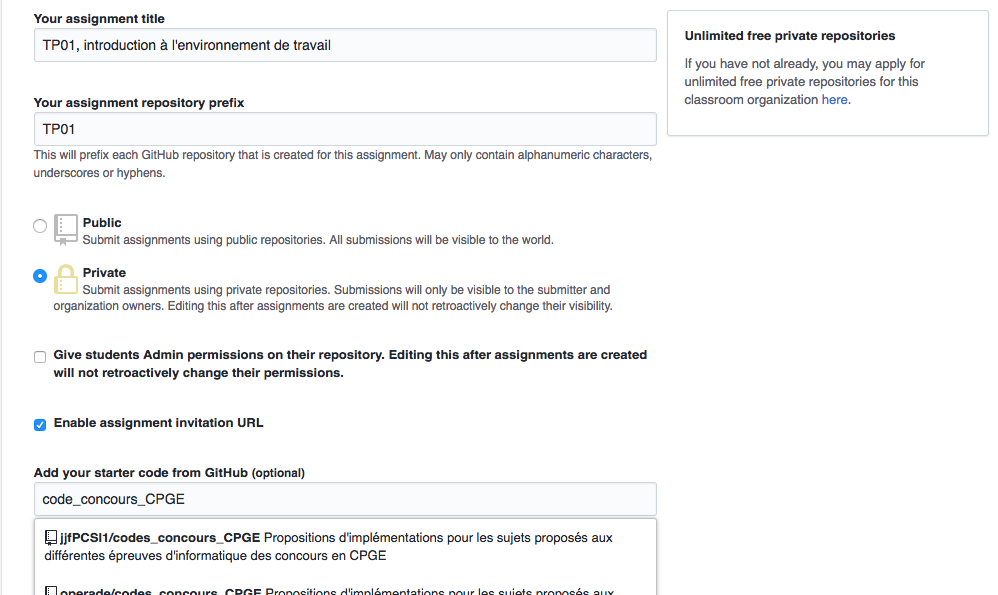
\includegraphics[height=0.8\textheight]{figures/classroom_assignment_reglages.png}
	\end{center}

\end{frame}

%%%%%%%%%%%%%%%%%%%%%%%%%%%%%%%%%%%%%%%%%%%%%%%%
%%%%%%%%%%%%%%%%%%%%%%%%%%%%%%%%%%%%%%%%%%%%%%%%
\begin{frame}
	\frametitle{Premier «Assignment»}
	\framesubtitle{Récupération des dossiers}

	\begin{center}
		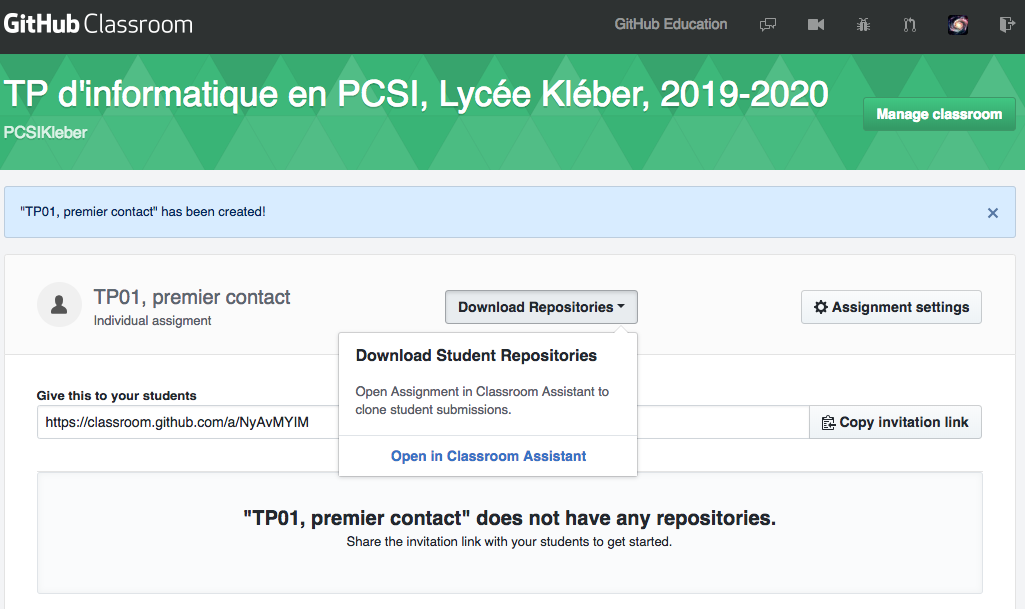
\includegraphics[width=\linewidth]{figures/classroom_assignment_suivi.png}
	\end{center}

\end{frame}
